\section{Codon IMM}

A protein can be modelled by a HMM with states that emit amino acids. For example,
\Cref{fig:core-model} shows a possible HMM architecture for aligning sequences of amino acids, for
which indels are modelled by insert ($\state{I}$) and delete ($\state{D}$) states and matched
positions are modelled by match ($\state{M}$) states. Each match state defines a potentially
distinct probability distribution over amino acids so as to model position-specific amino acid
frequencies. Insert states might instead define the same background probability distribution over
amino acids. Delete states are silent states and therefore do not emit any amino acid: it represents
position-specific missing amino acids. $\state{B}$ and $\state{E}$ are special states that represent
the end and start positions of an alignment. In particular, the probability of $\state{B}$ being the
first state is one: $p(Q_1=\state{B})=1$.

\begin{figure}[htbp]
  \centering
  \captionsetup{width=.5\linewidth}
  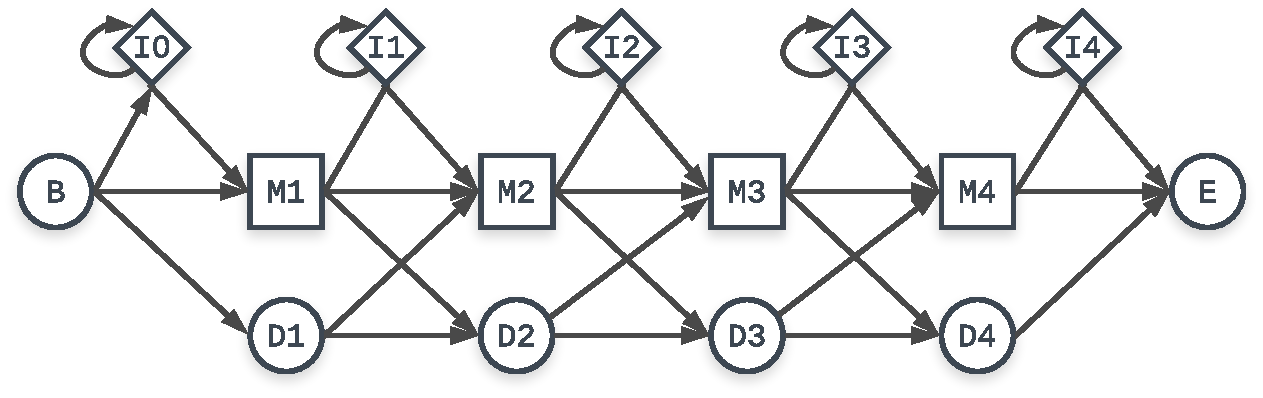
\includegraphics[width=.5\linewidth]{figure/core-model}
  \caption{HMM architecture for aligning sequences of four positions. $\state{B}$ and $\state{E}$
  are silent states denoting the start and the end positions of an aligment. States $\state{M}$
  represent matches while states $\state{I}$ and $\state{D}$ model indels.}\label{fig:core-model}
\end{figure}

HMMs are widely used to model proteins and are used to search for homologous subsequences in target
sequences made of amino acids. However, the researcher ocasionally do not have a ready-to-use amido
acid sequence but instead a sequence of nucleotides that might contain homologous subsequences that
code for proteins. Some nucleotides of those homologous subsquences might be missing or might have
been inserted by whatever reason. Still, one should be able to uncover error-prone subsequences when
compared against their homologous protein HMMs.

Let $(Q_t, S_t)$ be a HMM with the amino acid alphabet $\set{A}$ representing a protein profile. We
want to replace it by an IMM that preserves the model architecture (i.e., same set of states, state
transitions and initial state probabilities) but instead have states that emit sequences of
nucleotides instead of amino acid symbols. In particular, the new match and insert states will emit
nucleotide sequences that varies in length: from one to five nucleotides. The emission distribution
of silent states (e.g., delete states and special ones) will stay the same: probability one of
emitting an empty sequence in the IMM parlance. With such model, we hope to uncover error-prone
sequences of nucleotides that are homologous to protein profiles.

Let $\set{B}$ be a nucleotide alphabet (e.g., $\set{B} \eqdef \{\res{A}, \res{C}, \res{G},
\res{T}\}$), and let $\state{M}$ be a state that in the protein HMM would emit an amino acid. From
its amino acid distribution together with any other relevant source of information (codon usage
bias, for instance), one can define the probability $p(X_t=x_1x_2x_3 \gv Q_t=\state{M})$ of
$\state{M}$ emitting the codon $(x_1, x_2, x_3) \in \set{B}^3$.

\begin{example}
  Suppose that a state $\state{M}$ has the amino acid distribution defined by
  \begin{equation*}
    p(S_t=\res{Y} \gv Q_t=\state{M}) = 0.8 ~~\text{and}~~ p(S_t=\res{C} \gv Q_t=\state{M}) = 0.2,
  \end{equation*}
  where $\res{Y}$ and $\res{C}$ are the Tyrosine and Cysteine amino acids from the original alphabet
  $\set{A}$. Based on the canonical genetic code alone, we could define the codon distribution as
  follows:
  \begin{equation*}
    \begin{split}
      p(X_t=\res{TAT}\gv Q_t=\state{M})= 0.8/2, &\quad p(S_t=\res{TAC}\gv Q_t=\state{M})=0.8/2\\
      p(X_t=\res{TGT}\gv Q_t=\state{M})= 0.2/2, &\quad p(S_t=\res{TGC}\gv Q_t=\state{M})=0.2/2,
    \end{split}
  \end{equation*}
  where $\res{A}$, $\res{C}$, $\res{T}$, and $\res{G}$ are nucleotides from $\set{B}$.
\end{example}

Defining $p(X_t=x_1x_2x_3 \gv Q_t=q_t)$ as we did in the previous example for every state $q_t \in
\set{Q}$ of a given protein HMM produces an IMM $(Q_t, X_t)$ that instead emits codon sequences.
This model could in principle be used to evaluate sequences of nucleotides against the modelled
protein. However, such a model would fail to match sequences that present indels at the base level:
a match state that mainly emits Tyrosine (codons $\res{TAT}$ and $\res{TAC}$ in the canonical
genetic code) should be able to consider the sequence $\res{TAAT}$ as a possible Tyrosine codon that
happens to have a base insertion. We therefore propose an additional, crucial modification: the
emitted codon has to go through two steps of base deletions and two steps of base insertions. In
each of those steps, there will be a (small) probability $\e$ of a modification happening.
\Cref{fig:hmm-to-imm} summarizes the proposed modifications.

\begin{figure}[htbp]
  \centering
  \captionsetup{width=.5\linewidth}
  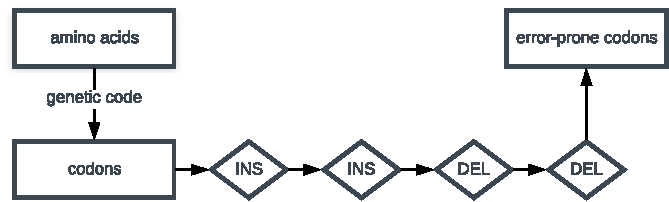
\includegraphics[width=.5\linewidth]{figure/hmm-to-imm}
  \caption{Conversion of protein HMM into codon IMM.\@ Amino acid distributions are first converted
  into codon distributions. Generated codons go through four indel steps, each of which has a
  probability $\e$ of actually modifiying the current sequence. At the end, we have a distribution
  of error-prone codons: variable-length sequences of one, two, three, four, or five
  nucleotides.}\label{fig:hmm-to-imm}
\end{figure}

The base-indel steps of our proposed mofication is graphically detailed in \Cref{fig:codon-hmm-tree}
and is further explained in the following. The deletion can happen in any of the three codon
positions with equal probability. If a deletion has already happened (i.e., the first deletion step
has indeed modified the emitted codon), the next deletion can happen in any of the remaining two
positions with equal probability. The insertion can happen between any two bases, before the first
base, or after the last base with equal probability. One remains to define the nucleotide
distribution of the insertion process, which we shall assume to have been established for now.

\subsection{Sequence distribution}

Let us assume that we already have the error-free codon distribution $p(X_t=x_1x_2x_3 \gv Q_t=q_t)$
from the amino acid distribution of state $q_t$. Given that a base insertion occurs, let $p(x)$
denote the probability of $x \in \set{B}$ being the inserted base. This section will formally define
the error-prone codon distribution $p(Z_t=z_1z_2\dots \gv Q_t=q_t)$ from distribution
$p(X_t=x_1x_2x_3 \gv Q_t = q_t)$ and parameter $\e$ based on the outlined method. We will omit the
index $t$ and the conditional part of the probability for simplicity. The next sections will also
use an underscore $\s$ to denote a summation over the corresponding sequence positions. For example,
$p(X=x_1\s\s)=\sum_{x_2,x_3}p(X=x_1x_2x_3)$.

\subsubsection{Sequences of length 1}

\begin{equation*}
  p(Z=z_1) = \e^2(1-\e)^2(p(X=z_1\s\s) + p(X=\s z_1\s) + p(X=\s\s z_1)) / 3
\end{equation*}

\subsubsection{Sequences of length 2}

\begin{equation*}
  \begin{split}
    p(Z=z_1z_2)
        &= 2\e(1-\e)^3(p(X=\s z_1z_2) + p(X=z_1\s z_2) + p(X=z_1z_2\s))/3\\
        &+ \e^3(1-\e)(p(X=z_1\s\s) + p(X=\s z_1\s) + p(X=\s\s z_1))p(z_2)/3\\
        &+ \e^3(1-\e)(p(X=z_2\s\s) + p(X=\s z_2\s) + p(X=\s\s z_2))p(z_1)/3
  \end{split}
\end{equation*}

\subsubsection{Sequences of length 3}

\begin{equation*}
  \begin{split}
    p(Z=z_1z_2z_3) &= (1-\e)^4 p(X=z_1z_2z_3)\\
        &+ 4\e^2(1-\e)^2 (p(X=\s z_2 z_3) + p(X=z_2\s z_3) + p(X=z_2 z_3\s))p(z_1)/9\\
        &+ 4\e^2(1-\e)^2 (p(X=\s z_1 z_3) + p(X=z_1\s z_3) + p(X=z_1 z_3\s))p(z_2)/9\\
        &+ 4\e^2(1-\e)^2 (p(X=\s z_1 z_2) + p(X=z_1\s z_2) + p(X=z_1 z_2\s))p(z_3)/9\\
        &+ \e^4 (p(X=z_3\s\s) + p(X=\s z_3\s) + p(X=\s\s z_3))p(z_1)p(z_2)/9\\
        &+ \e^4 (p(X=z_2\s\s) + p(X=\s z_2\s) + p(X=\s\s z_2))p(z_1)p(z_3)/9\\
        &+ \e^4 (p(X=z_1\s\s) + p(X=\s z_1\s) + p(X=\s\s z_1))p(z_2)p(z_3)/9
  \end{split}
\end{equation*}

\subsubsection{Sequences of length 4}

\begin{equation*}
  \begin{split}
    p(Z=z_1z_2z_3z_4) &= \e(1-\e)^3 (p(X=z_2z_3z_4)p(z_1)+p(X=z_1z_3z_4)p(z_2)\\
        &+p(X=z_1z_2z_4)p(z_3)+p(X=z_1z_2z_3)p(z_4))/2\\
        &+\e^3(1-\e)(\\
        &+ p(X=\s z_3z_4)p(z_1)p(z_2) + p(X=\s z_2z_4)p(z_1)p(z_3)\\
        &+ p(X=\s z_2z_3)p(z_1)p(z_4) + p(X=\s z_1z_4)p(z_2)p(z_3)\\
        &+ p(X=\s z_1z_3)p(z_2)p(z_4) + p(X=\s z_1z_2)p(z_3)p(z_4)\\
        &+ p(X=z_3\s z_4)p(z_1)p(z_2) + p(X=z_2\s z_4)p(z_1)p(z_3)\\
        &+ p(X=z_2\s z_3)p(z_1)p(z_4) + p(X=z_1\s z_4)p(z_2)p(z_3)\\
        &+ p(X=z_1\s z_3)p(z_2)p(z_4) + p(X=z_1\s z_2)p(z_3)p(z_4)\\
        &+ p(X=z_3z_4\s)p(z_1)p(z_2) + p(X=z_2z_4\s)p(z_1)p(z_3)\\
        &+ p(X=z_2z_3\s)p(z_1)p(z_4) + p(X=z_1z_4\s)p(z_2)p(z_3)\\
        &+ p(X=z_1z_3\s)p(z_2)p(z_4) + p(X=z_1z_2\s)p(z_3)p(z_4))/9
  \end{split}
\end{equation*}

\subsubsection{Sequences of length 5}

\begin{equation*}
  \begin{split}
    p(Z=z_1z_2z_3z_4z_5)
        &= \e^2(1-\e)^2(\\
        &+p(z_1)p(z_2)p(X=z_3z_4z_5)+p(z_1)p(z_3)p(X=z_2z_4z_5)\\
        &+p(z_1)p(z_4)p(X=z_2z_3z_5)+p(z_1)p(z_5)p(X=z_2z_3z_4)\\
        &+p(z_2)p(z_3)p(X=z_1z_4z_5)+p(z_2)p(z_4)p(X=z_1z_3z_5)\\
        &+p(z_2)p(z_5)p(X=z_1z_3z_4)+p(z_3)p(z_4)p(X=z_1z_2z_5)\\
        &+p(z_3)p(z_5)p(X=z_1z_2z_4)+p(z_4)p(z_5)p(X=z_1z_2z_3))/10
  \end{split}
\end{equation*}

\subsection{Codon decoding}

Note that
\begin{equation*}
  p(X=x_1x_2x_3 \gv Z=\arr{z}) \propto p(Z=\arr{z} \gv X=x_1x_2x_3) p(X=x_1x_2x_3).
\end{equation*}
It therefore remains to compute
\begin{equation*}
  p(Z=\arr{z} \gv X=x_1x_2x_3) = \sum_{\pi}p(Z=\arr{z} \gv \Pi=\pi, X=x_1x_2x_3) p(\Pi=\pi),
\end{equation*}
for which $\pi$ is a path of the base-indel process.

We have

\subsubsection{Sequences of length 1}

\begin{equation*}
  p(Z=z_1 \gv X=x_1x_2x_3) = \e^2(1-\e)^2(\I(x_1, z_1) + \I(x_2, z_1) + \I(x_3, z_1))/3
\end{equation*}

\subsubsection{Sequences of length 2}

\begin{equation*}
  \begin{split}
    p(Z=z_1z_2 \gv X=x_1x_2x_3)
        &= 2\e(1-\e)^3(\I(x_2, z_1)\I(x_3, z_2) + \I(x_1, z_1)\I(x_3, z_2) + \I(x_1, z_1)\I(x_2, z_2))/3\\
        &+ \e^3(1-\e)(\I(x_1, z_1) + \I(x_2, z_1) + \I(x_3, z_1))p(z_2)/3\\
        &+ \e^3(1-\e)(\I(x_1, z_2) + \I(x_2, z_2) + \I(x_3, z_2))p(z_1)/3
  \end{split}
\end{equation*}

\subsubsection{Sequences of length 3}

\begin{equation*}
  \begin{split}
    p(Z=z_1z_2z_3) &= (1-\e)^4 (1-\e)^4\I(x_1, z_1)\I(x_2, z_2)\I(x_3, z_3)\\
        &+ 4\e^2(1-\e)^2 (\I(x_2, z_2)\I(x_3, z_3) + \I(x_1, z_2)\I(x_3, z_ 3) + \I(x_1, z_2)\I(x_2, z_3)) p(z_1)/9\\
        &+ 4\e^2(1-\e)^2 (\I(x_2, z_1)\I(x_3, z_3) + \I(x_1, z_1)\I(x_3, z_3) + \I(x_1, z_1)\I(x_2, z_3))p(z_2)/9\\
        &+ 4\e^2(1-\e)^2 (\I(x_2, z_1)\I(x_3, z_2) + \I(x_1, z_1)\I(x_3, z_2) + \I(x_1, z_1)\I(x_2, z_2))p(z_3)/9\\
        &+ \e^4 (\I(x_1, z_3) + \I(x_2, z_3) + \I(x_3, z_3))p(z_1)p(z_2)/9\\
        &+ \e^4 (\I(x_1, z_2) + \I(x_2, z_2) + \I(x_3, z_2))p(z_1)p(z_3)/9\\
        &+ \e^4 (\I(x_1, z_1) + \I(x_2, z_1) + \I(x_3, z_1))p(z_2)p(z_3)/9
  \end{split}
\end{equation*}

\subsubsection{Sequences of length 4}

\subsubsection{Sequences of length 5}

\subsection{Analysis}

The codon emitted at node $\state{M}$ in \Cref{fig:codon-hmm-tree} can go through $m\in\{0, 1, 2, 3,
4\}$ base indels during the node transitions that end at some leaf-node. The probability of
it undergoing $m$ indels is given by
\begin{equation*}
  p(M=m) = \binom{4}{4-m} (1 - \e)^{4-m} \e^m,
\end{equation*}
where the coefficient $\binom{4}{m}$ counts the number of paths corresponding to $m$ base indels.
\Cref{fig:indel-dist} shows the base indel distributions over different values of $\e$.
Let $F$ be a random variable representing the final sequence length generated by the model in
\Cref{fig:codon-hmm-tree}.
We have the probabilities
\begin{equation*}
  \begin{split}
    p(F=1) = p(F=5) &= \e^2(1-\e)^2, \\
    p(F=2) = p(F=4) &= 2\e^3(1-\e) + 2\e(1-\e)^3,~\text{and} \\
    p(F=3)          &= \e^4 + 4\e^2(1-\e)^2 + (1-\e)^4,
  \end{split}
\end{equation*}
illustrated in \Cref{fig:len-dist} over different values of $\e$.

\begin{figure}[htbp]
  \centering
  \captionsetup{width=0.85\linewidth}
  \begin{subfigure}{.5\linewidth}
    \centering
    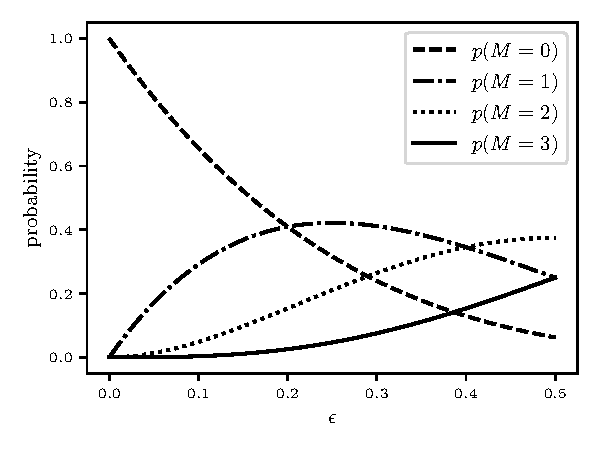
\includegraphics[width=.7\linewidth]{figure/indel-prob}
    \caption{Base indel distribution.}\label{fig:indel-dist}
  \end{subfigure}%
  \begin{subfigure}{.5\linewidth}
    \centering
    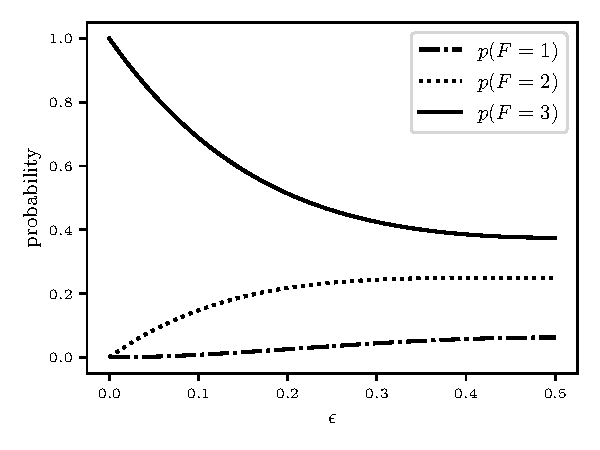
\includegraphics[width=.7\linewidth]{figure/seq-len-prob}
    \caption{Sequence length distribution.}\label{fig:len-dist}
  \end{subfigure}
  \caption{ Distribution of base indels and sequence length over the modification probability
  $\e$. It seems reasonable to choose a $\e$ value that is smaller than $1/5$ such that
  $p(M=m)<p(M=m+1)$, as per \Cref{fig:indel-dist}. }\label{fig:dist}
\end{figure}

\newpage
\begin{sidewaysfigure}[ht]
    \centering
    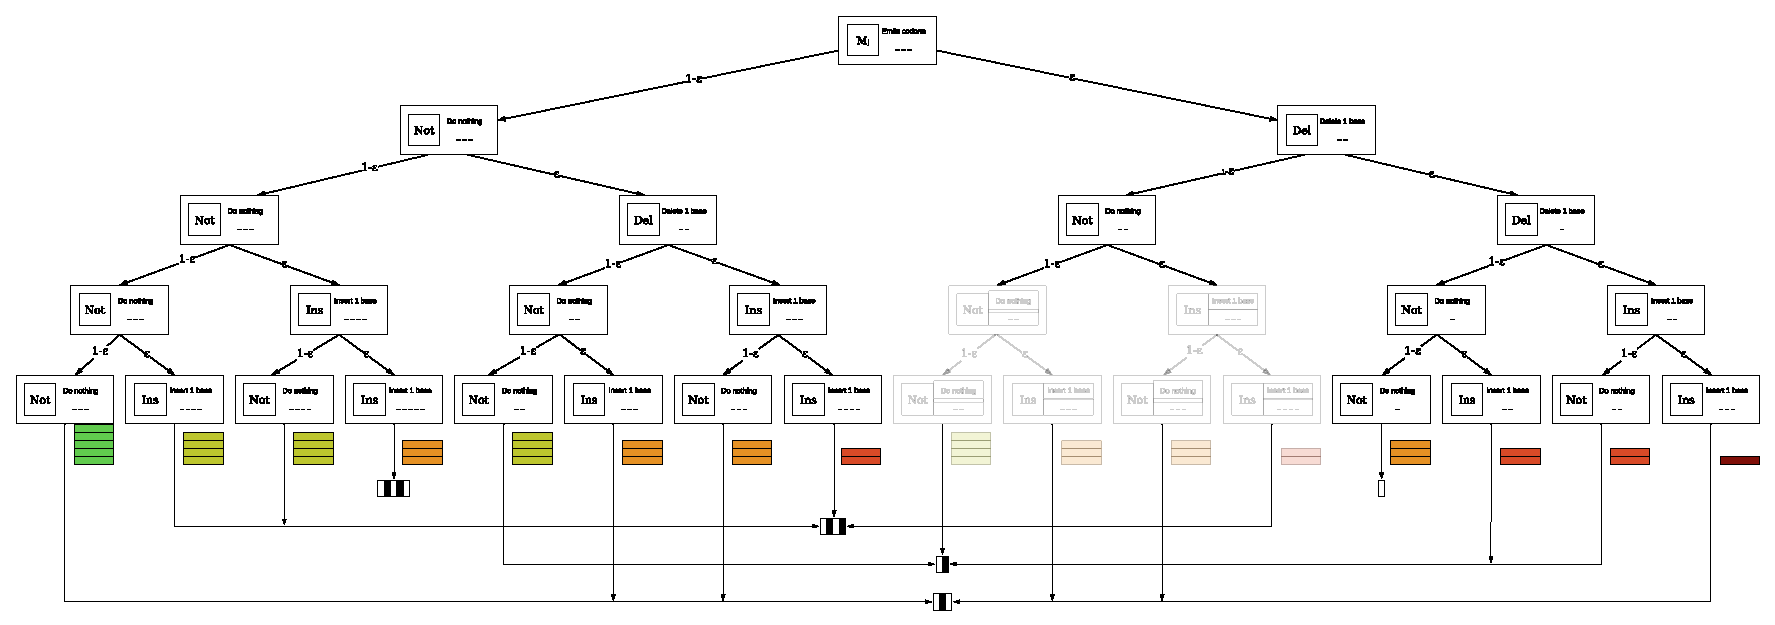
\includegraphics[scale=0.9]{figure/codon-hmm-tree}
    \caption{Matched codon HMM tree.
        The $\e$-transitions occur infrequently and exist to account for sequence errors.
        The most probably path ends at the first leaf-node from left to right.}\label{fig:codon-hmm-tree}
\end{sidewaysfigure}
